\documentclass{article}

\usepackage{multicol}
\usepackage{authblk}
\usepackage{blindtext}
\usepackage{graphicx}
\usepackage{booktabs}
\usepackage{placeins}
\usepackage{siunitx}
\usepackage[a4paper, total={7in, 10in}]{geometry}
\usepackage[colorlinks,citecolor=blue,urlcolor=red,bookmarks=false,hypertexnames=true]{hyperref}
\usepackage{amsmath}
\usepackage{academicons}
\usepackage{xcolor}

\newbox{\myorcidaffilbox}
\sbox{\myorcidaffilbox}{\large
\includegraphics[height=1.7ex]{imgs/ORCIDiD_icon16x16.png}}

\newcommand{\orcidaffil}[1]{%
	\href{https://orcid.org/#1}{\usebox{\myorcidaffilbox}}}

\newcommand{\showorcidaffil}[1]{%
	\href{https://orcid.org/#1}{\usebox{\myorcidaffilbox}}#1}

\newcommand{\icol}[1]{% inline column vector
	\left(\begin{bmatrix}#1\end{bmatrix}\right)%
}

\newcommand{\irow}[1]{% inline row vector
	\begin{bmatrix}#1\end{bmatrix}%
} 


\author[1]{Author1 \orcidaffil{0000-0000-0000-0000}}
\author[1]{Author2 \orcidaffil{0000-0000-0000-0000}}
\author[2]{Author3 \orcidaffil{0000-0000-0000-0000}}
\affil[1]{Author Affiliation1 }
\affil[2]{Author Affiliation2}
\affil[ ]{\textit {\{email1,email2,email3,email4,email5\}@xyz.edu}}

\begin{document}
	\title{Report Title}	
	
	\maketitle
	
	\begin{abstract}
		The body of your abstract begins here. It should be an explicit summary of your presentation that
		states the problem, the methods used, and the major results and conclusions. Do not include scientific symbols,
		acronyms, numbers, bullets or lists in the abstract. It should be single-spaced in 10-point Times New Roman.
		The first part of your abstract should state the problem you set out to solve or the issue you set out to explore
		and explain your rationale for pursuing the project. The problem or issue might be a research question, a gap in
		critical attention to a text, a societal concern, etc. The purpose of your study is to solve this problem and/or add
		to your discipline’s understanding of the issue. This section of the abstract should explain how you went about
		solving the problem or exploring the issue you identified. Your abstract should also describe the research
		methods; this section should include a concise description of the process by which you conducted your research.
		Next, your abstract should list the results or outcomes of the work you have done so far. If your project is not
		yet complete, you may still include preliminary results or your hypotheses about what those results will
		be. Finally, your abstract should close with a statement of the project’s implications and contributions to its
		field. It should convince readers that the project is interesting, valuable, and worth investigating further. In
		particular, it should convince conference registrants to attend your presentation. These directions are written in
		the format required for the abstract of the paper for the Center for Scholastic Inquiry’s International Academic
		Research Conferences. We recommend that you download these directions as a MS Word document and use it
		as the template for your abstract as it contains all necessary formats and styles. The content of the abstract will
		be the basis for acceptance of the paper presentation at the international research conference. The abstracts will
		be peer reviewed and authors will be informed about acceptance for presentation via email. Be sure to adhere to
		the word limitation for the abstract (250 words).
	\end{abstract}
	
	\section{Section with HyperLink}
	\href{https://www.sciencedirect.com/topics/medicine-and-dentistry/image-registration}{Image registration} is defined as a process that overlays two or more images from various imaging equipment or sensors taken at different times and angles, or from the same scene to geometrically align the images for analysis. 
	\section{Section with Item}
	\begin{itemize}
		\item Item1
		\item Item2
		\item Item3
	\end{itemize}
	\section{Section with Equation}
	The problem of using histogram vector is that histogram feature vector is not a vector in Euclidean Space. Therefore a histogram distance formula is proposed as the intersection between two distribution. Consider two distribution histogram $H(I)$ and $H(I\prime)$ calculated from two images $I$ and $I\prime$. Since $H(I)$ and $(I\prime)$ have the same bin $n$, the normalized histogram is calculated in the Equation \ref{eq:hiscap}:
	\begin{equation}
		H(I) \cap H(I\prime) = \sum_{j = 1}^{n}min(H_j(I), H_j(I\prime))
		\label{eq:hiscap}
	\end{equation}
	\section{Section with Citation}
	There has been many researches using feature descriptor over the last decade. Hirokazu et al proposes a method of retrieving multi-scale objects from optical colonoscopy images based on image recognition techniques \cite{7348442}. The proposed method is a method of content-based image retrieval (CBIR). \cite{7348442} improves the geometric feature extraction component in order to handle the retrieval of multi-scale objects	by utilizing the integral image technique \cite{207-212}. In this research, both object size and	object color are considered as points of contrast, because the illumination conditions for each image are a function of the focal distance. For preprocessing, we adopt the saturation element converted from the original colonoscopy images for the	RGB color space. In addition, bright blobs within colonic
	images are interpolated by a method of image inpainting \cite{25-36}
	prior to conversion, because the saturation element cannot be
	converted from bright blobs. In this study, a feature extraction method formed by the combination of HALC \cite{halc} and Integral Image Technique \cite{25-36} are proposed. 
	\section{Section with Image}
	\FloatBarrier
	\begin{figure}[h]
		\caption{Wavelet Transform step. (a) First step of the DWT for a signal of length 16. (b) Second step of the DWT.}
		\centering
		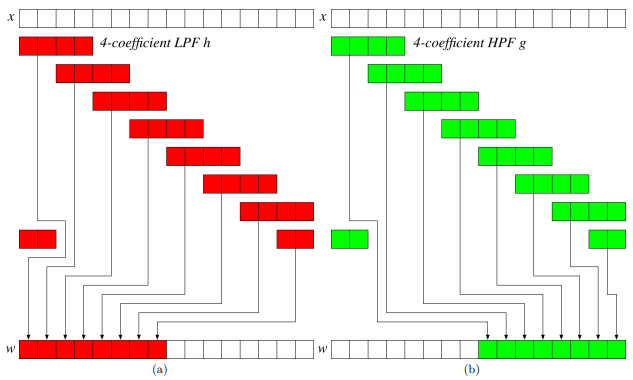
\includegraphics[width=0.7\textwidth]{imgs/waveletstep}
		\label{fig:waveletstep}
	\end{figure}
	\FloatBarrier
	
	%Biliography Rendering
	\bibliographystyle{ieeetr} 
	\bibliography{ref} 
	
	%Appendix Starting
	\appendix

\end{document}



